
\section{Background}

In this section, we provide a brief introduction to contact modeling with the
linear complementarity formulation.
%
We also present a summary of the mixture of experts architecture and
its uses in machine learning.
%
In Section~\ref{sec:moe_methods}, we utilize the high-fidelity models obtained
from the linear complementarity formulation in order to design contact-aware
mixture of expert controllers through data-driven techniques.

\subsection{Contact Modeling with Linear Complementarity Problem}

Suppose a hybrid dynamical system consists of $k$ potential contacts, each
introducing normal contact forces $\lambda_N \in \mathbb{R}^{k}$ and Coulomb
friction forces $\lambda_T \in \mathbb{R}^{k}$ to the overall system.
%
The contact forces in this hybrid system enforce the geometric and kinematic
constraints of surfaces in contact.
%
For instance, the contact force between two objects in collision characterizes
the no-penetration conditions and the post-impact velocities of the objects.
%
An accurate contact model identifies the contact forces necessary to obey these
kinematic constraints, however resolving the contact forces accurately can be
difficult and computationally expensive.
%
Most collision simulators work on the kinematic level as opposed to the dynamic
level.
%
For instance, there are event detection methods~\cite{cellier1986combined} that
simply change the velocity of the moving objects at the time of impact.
%
One of the drawbacks of these techniques is finding the exact time the contact
occurs in high speed collision.
%
There is the additional difficulty of identifying the Coulomb friction.
% , which is
% especially prone to Painlev{{\'e}} Paradox~\cite{genot1999new} in high friction
% scenarios.
%
The linear complementarity formulation in~\cite{glocker2005formulation} provides
a rigorous technique to resolve contact forces, Coulomb friction and impact
forces in a hybrid system.
%
This formulation presents an optimization problem that searches for \it{contact force
and post-impact velocity} \normalfont pairs that obey the geometric and
kinematic constraints during contacts or impacts.
%

%
The linear complementarity formulation is constructed from kinematic and dynamic
constraints of contact, which we discuss as follows.
%
We begin by introducing the variables necessary to define the kinematic
constraints of a contact-rich system.
%
Suppose we have a contact-rich mechanism whose states $x \in \mathcal{X} \subset
\mathbb{R}^{2m}$ consists of generalized positions $q \in \mathbb{R}^m$ and
velocities $\dot{q}$.
%
Let $g_N(q) \in \mathbb{R}^{k}$ denote a vector of gap functions that measure
the normal distance between the contact surfaces. 
%
The normal and tangential relative velocities between the contact surfaces are
given by $\gamma_N = \dot{g}_N(q)$ and $\gamma_T$, respectively.
%
We can express the relative velocities $\gamma_N$ and $\gamma_T$ in terms of the
generalized velocities as 
%
\begin{align}
  \gamma_N = W_N \dot{q}, \; \gamma_T = W_T \dot{q},
  \label{eq:gamma}
\end{align}  
\noindent where $W_N$ and $W_T$ are the linear mappings from the generalized
coordinates to the local contact coordinates.
%
The kinematic constraints of contact provide a connection between pre- and
post-impact velocities throughout this formulation, thus we introduce the
following notations.
%
The pre- and post-impact generalized velocities are denoted by $\dot{q}^-$ and
$\dot{q}^+$, respectively, and their corresponding relative velocities are given
by
\begin{align*}
  \gamma_N^+ = W_N\dot{q}^+, \; \gamma_T^+ = W_T\dot{q}^-, \\
  \gamma_N^- = W_N\dot{q}^-, \; \gamma_T^- = W_T\dot{q}^-.
\end{align*}
%
The kinematic constraint of contact states that two rigid bodies undergoing
contact must always maintain a normal distance such that $g_N \geq 0$. Moreover,
in the presence of contacts, the post-impact velocities can be found from the
pre-impact velocities as:
\begin{align}
  \begin{gathered}
    \gamma_N^+ = -\epsilon_N \gamma_N^-, \\
    \gamma_T^+ = -\epsilon_T \gamma_T^-,
  \end{gathered}
  \label{eq:postimpactVel}
\end{align}
\noindent where $\epsilon_N \in \mathbb{R}^k$ and $\epsilon_T \in \mathbb{R}^k$
are diagonal matrices consisting of the normal and tangential coefficients of
restitution, respectively.

%
The dynamic constraints of contact-rich system are given by the
model~\cite{glocker2005formulation}
\begin{equation}
  \begin{gathered}
    M(q) \dd \dot{q} + h(q, \dot{q})\dd t - \dd R  = 0, \\
    h(q, \dot{q}) = C(q, \dot{q})\dot{q} + G(q) - Bu(q, \dot{q}), 
    \end{gathered}
  \label{eq:hybrid_dynamics}
\end{equation}
%
\noindent where $M \in \mathbb{R}^{m \times m}$ denotes the positive-definite
mass matrix, $C \in \mathbb{R}^{m \times m}$ holds the Coriolis and centripetal
terms, and $G \in \mathbb{R}^{m}$ is the gravitational term. The matrix $B \in
\mathbb{R}^{m \times n}$ maps the input $u \in \mathcal{U} \subset
\mathbb{R}^{n}$ to the generalized coordinates.
%
The force measure $\dd R$ contains the contact forces as 
\begin{align*}
    \dd R = W_N \dd \lambda_N + W_T \dd \lambda_T ,
\end{align*}
\noindent where $W_N$ and $W_T$ are the projection matrices that map the effect
of the normal and tangential contact forces, respectively, to the generalized
coordinates.
%
The vectors $\dd \lambda_N$ and $\dd \lambda_T$
consist of the normal and tangential contact impulse measures, respectively.
%
In the presence of impacts, we integrate the contact measures over a singleton
time $t$ as $\int_{\{t\}} (\dd \lambda_N , \dd \lambda_T) = (\lambda_N(t),
\lambda_T(t))$ in order to obtain the impulsive contact forces.
%
In the case of persisting contact forces, the contact impulse measures evaluate
to $(\dd \lambda_N, \dd \lambda_T) = (\dot{\lambda}_N, \dot{\lambda}_T)$, where
$\dot{\lambda}_N$ and $\dot{\lambda}_T$ hold the normal and the tangential contact
forces, respectively.
%
The dynamic constraint in~\eqref{eq:hybrid_dynamics} characterizes how the
local contact forces affect the dynamics of the overall system.
\begin{rem}
  Unlike the classical second order equations of motion $M(q) \ddot{q} + h(q,
  \dot{q}) = 0$, the measure differential inclusion
  in~\eqref{eq:hybrid_dynamics} can characterize the behavior of the system
  under impact forces. Notice that in the presence of impacts, the velocity
  $\dot{q}$ is not continuous for all time, thus the acceleration $\ddot{q}$
  does not exist everywhere. For further understanding of how the measure
  equality can accurately represent the impact dynamics, we refer the reader
  to~\cite{moreau1988unilateral}.
\end{rem}

We first motivate the linear complementarity formulation for normal contact
forces, where the system has no Coulomb friction.
% 
The linear complementarity formulation imposes a unilateral constraint between
contact forces and relative velocities given by:
\begin{equation}
  \begin{gathered}
    0 \leq 
      \xi_N(q, \dot{q}) 
      \perp
      \lambda_N  
      \geq 0, \\
  % \end{eqnarray}
  % \begin{eqnarray}
      \xi_N(q, \dot{q}) := \gamma_N^+ + \epsilon_N \gamma_N^-.
  \end{gathered}
  \label{eq:complementarity} 
\end{equation}
\noindent where $0 \leq a \perp b \geq 0$ denotes $a \geq 0, b \geq 0$ and
$a^\top b=0$.
% 
The physical interpretation of~\eqref{eq:complementarity} can be given as
follows.
%
% We first look at the properties of normal contact forces and relative velocities
% during contacts, and we translate the same concept to the tangential direction.
%
In the presence of contacts and impacts, the post-impact velocities can be found
from pre-impact velocities by~\eqref{eq:postimpactVel}.
%
In this scenario, the quantity $\xi_N$ evaluates to zero, because
\begin{align*}
  \xi_N &= \gamma_N^+ + \epsilon_N \gamma_N^- = -\epsilon_N \gamma_N^- + \epsilon_N \gamma_N^- = 0.
\end{align*}
%
The complementarity constraint in~\eqref{eq:complementarity} states that when
two surfaces come into contact, the resultant between pre- and post-impact
velocities, given by $\xi_N$ must be zero, and in the meantime, the contact
forces can take positive values.
%
Conversely, if there are no potential contacts, the relative velocities are
continuous, i.e. $\gamma_N^+ = \gamma_N^- = \gamma_N$.
%
In this case, the complementarity constraint states that $\xi_N$ can be
non-zero, which is analogues to contact surfaces approaching each other or
moving away from each other, but the normal contact forces $\lambda_N$ must be
zero. 
%
There exists no scenario when both the contact force $\lambda_N$ and $\xi_N$ are
both positive, hence $\xi_N^\top \lambda_N = 0$ must always hold.
%
This concept is summarized as shown in Table~\ref{tab:complementarity}.

\begin{table}[tb]
  \centering
  \caption{Linear Complementarity Formulation: Possible contact scenarios}
  \begin{tabular}{|c|c|c|c|c|c|}
    \hline
    Scenario & $g_N$ & $\gamma_N^-$ & $\gamma_N^+$ & $\xi_N$ & $\lambda_N$ \\
    \hline\hline
    No contact & $g_N \leq 0$  & $\gamma_N > 0$ & $\gamma_N$ & $ \gamma_N +\epsilon_N\gamma_N$ & $0$ \\
    Contact or impact & $g_N \leq 0$ &  $\gamma_N \leq 0$ & $- \epsilon_N \gamma_N$ & $0$ & $\lambda_N \geq 0$ \\
    \hline
  \end{tabular}
  \label{tab:complementarity}
\end{table}

\begin{figure}[b]
  \centering
  \begin{tikzpicture}
      \node [](image) at (0,0) {
          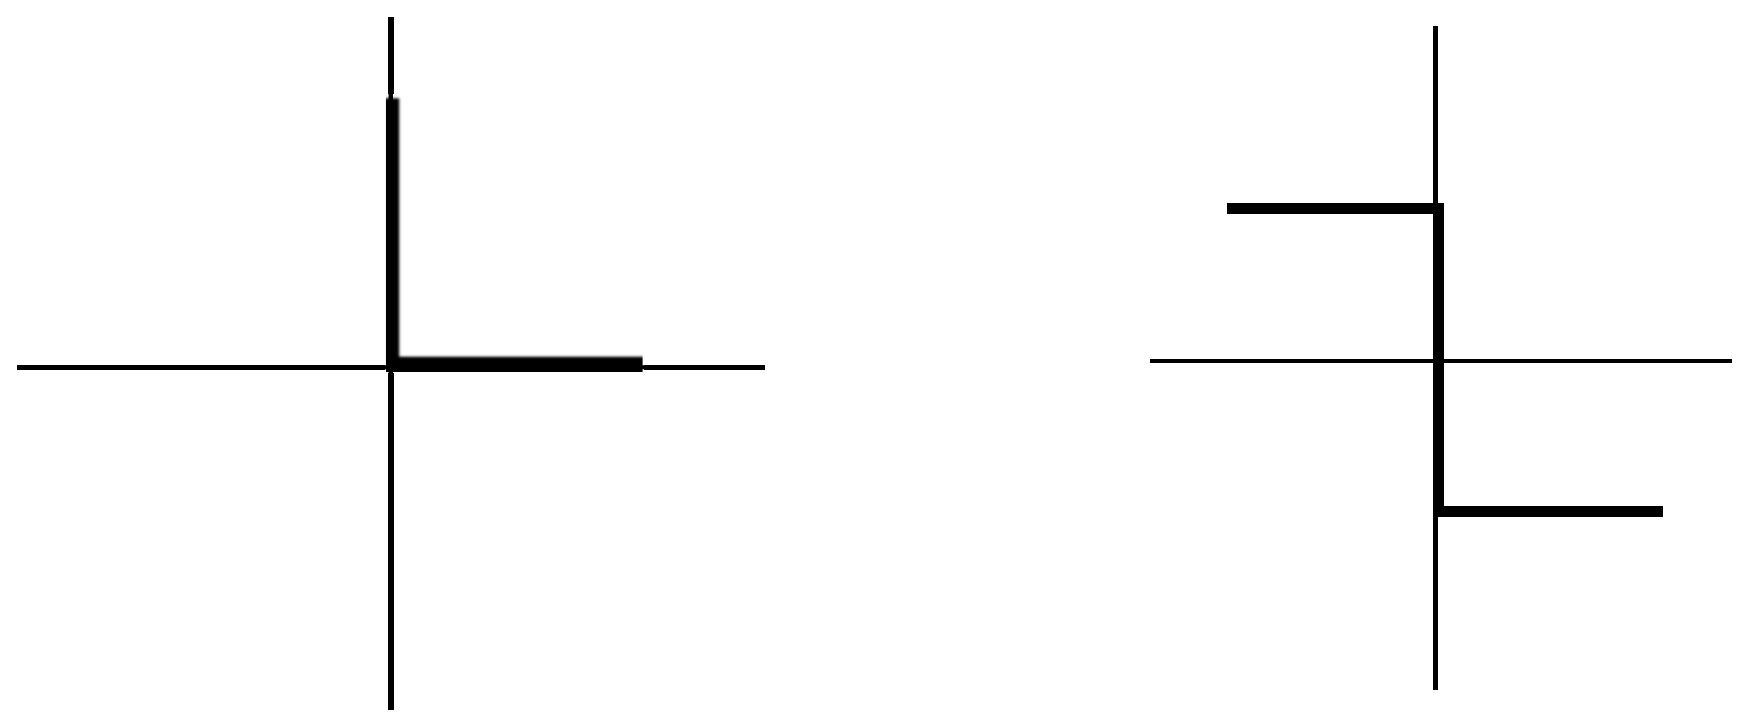
\includegraphics[width=0.6\textwidth]{unilateral_primitive.eps}
      };
      \node[] at (-2.3, 2.0) {\small $\lambda_N$};
      \node[] at (-1.0, -0.3) {\small $\xi_N$};
      \node[] at (3.6, 2.0) {\small $\lambda_T$};
      \node[] at (5.0, -0.3) {\small $\xi_T$};
      \node[] at (3.8, 1.2) {\small $\mu \lambda_N$};
      \node[] at (2.5, -1.0) {\small $-\mu \lambda_N$};
      % \draw[-stealth, dotted, very thick,black] (-0.7,-1.8) -- ++(1.2,5.0) node[above right,black,fill=white]{\small $\hat{n}$};
  \end{tikzpicture}
  \caption{Left: Complementarity condition for normal contact forces. Right: Characteristics of Coulomb friction as a function of $\xi_T$}
  \label{fig:unilateral_primitive}
\end{figure}
%
\begin{figure}
  \centering
  \begin{tikzpicture}
      \node [](image) at (0,0) {
          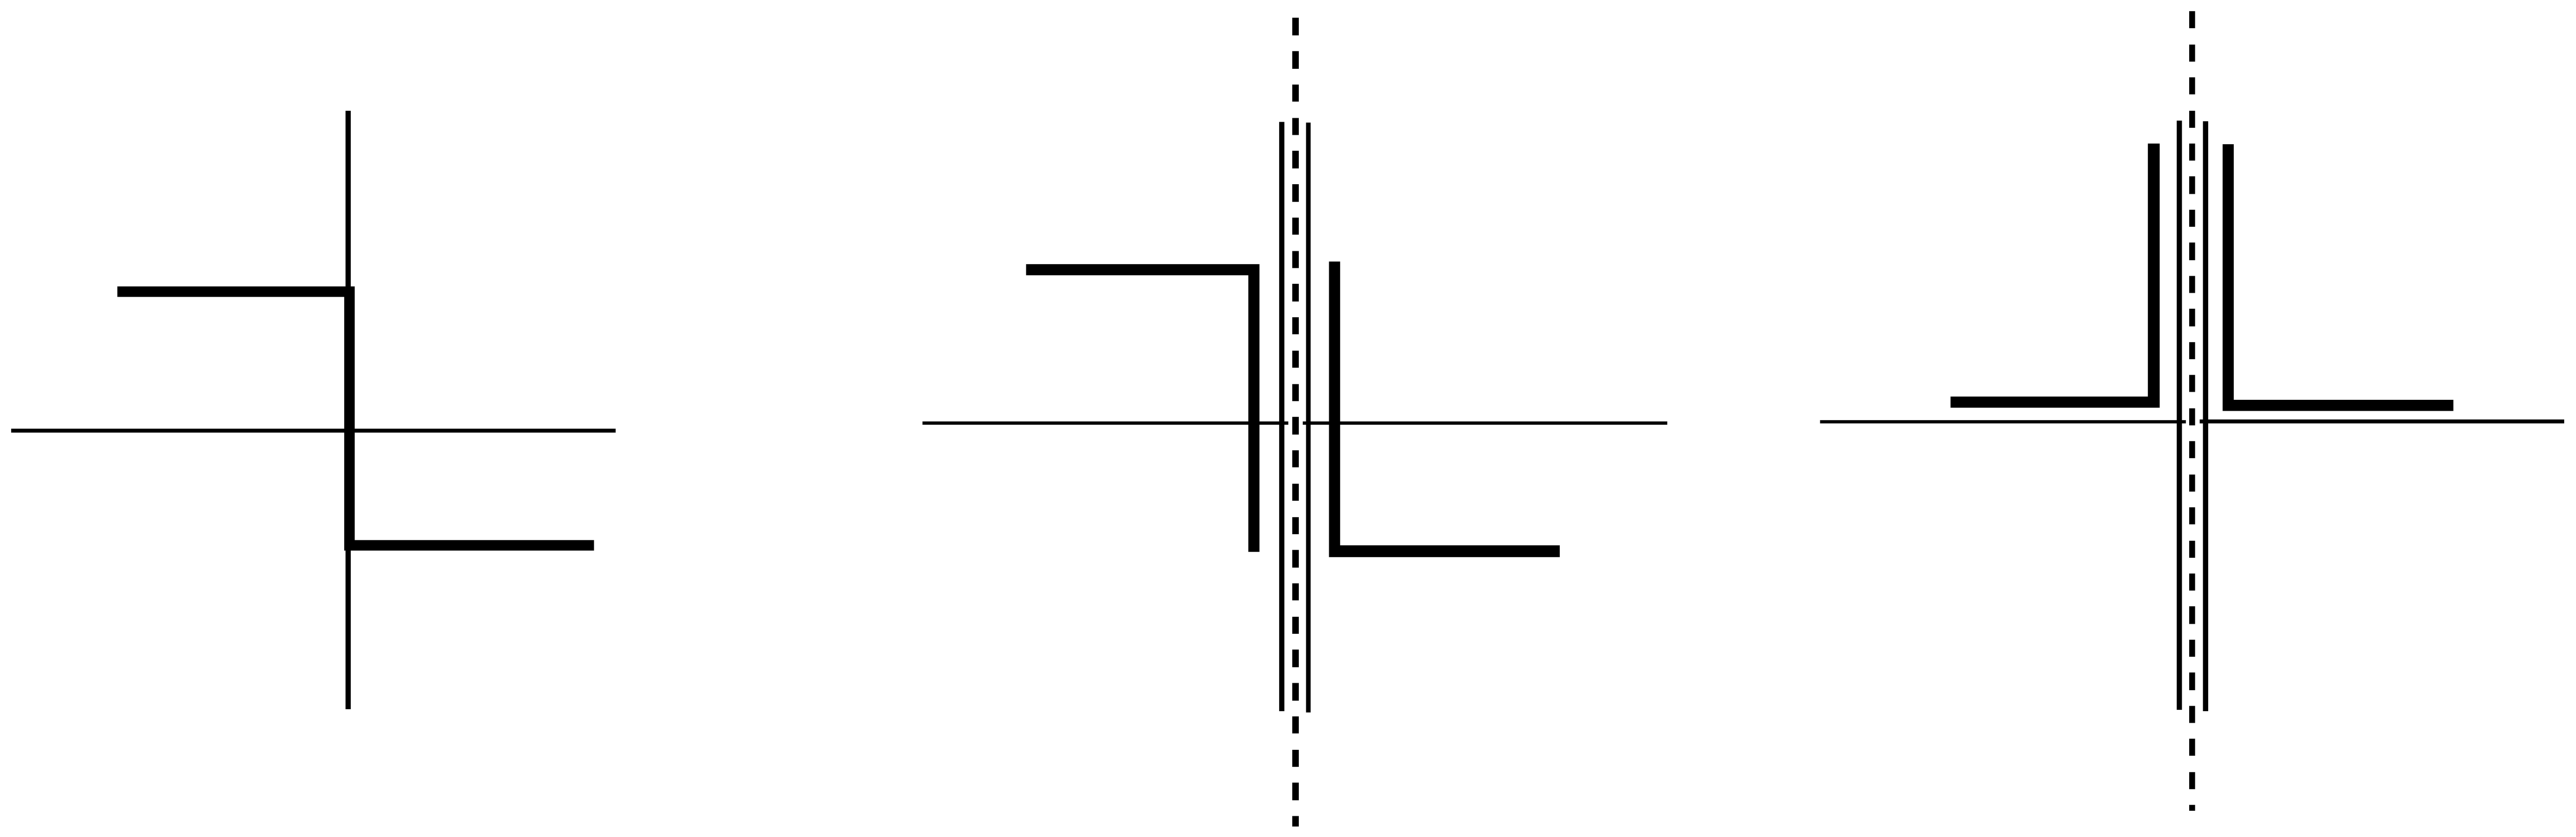
\includegraphics[width=0.9\textwidth]{tangential_to_complementary.eps}
      };
      \node[] at (-5.1, 1.8) {\small $\lambda_T$};
      \node[] at (-4.0, -0.4) {\small $\xi_T$};
      \node[] at (0.2, 2.0) {\small $\lambda_T$};
      \node[] at (-1.9, -0.3) {\small $\xi_L$};
      \node[] at (1.9, -0.3) {\small $\xi_R$};
      \node[] at (3.8, 2.0) {\small $\lambda_L = \mu \lambda_N - \lambda_T$};
      \node[] at (7.0, 2.0) {\small $\lambda_R = \mu \lambda_N + \lambda_T$};
      \node[] at (3.8, -0.3) {\small $\xi_L$};
      \node[] at (7.6, -0.3) {\small $\xi_R$};
      % \draw[-stealth, dotted, very thick,black] (-0.7,-1.8) -- ++(1.2,5.0) node[above right,black,fill=white]{\small $\hat{n}$};
  \end{tikzpicture}
  \caption{Construction of complementarity condition for Coulomb friction}
  \label{fig:tangential_to_complementarity}
\end{figure}

From \eqref{eq:gamma} and~\eqref{eq:hybrid_dynamics}, we can express $\xi_N$
as 
\begin{align*}
  \xi_N &= W_N^\top \dot{q}^+ + \epsilon_N W_N^\top \dot{q}^-, \\
  &= W_N^\top M^{-1}[-h \Delta t + W_N \lambda_N] + (1 + \epsilon_N)W_N^\top \dot{q}^-, \\
  &= \underbrace{W_N^\top M^{-1}W_N}_{A_N} \lambda_N \underbrace{-W_N^\top M^{-1}h \Delta t + (1 + \epsilon_N) W_N^\top \dot{q}^-}_{b_N}, \\
  &= A_N \lambda_N + b_N,
\end{align*}
\noindent where $\dot{q}^-$ and $\dot{q}^+$ represent the pre- and post-impact
velocities of the system, and $\Delta t$ is the integration time-step for the
discretization of~\eqref{eq:hybrid_dynamics}.
%
Notice that $\xi_N$ is a linear function of the contact forces $\lambda_N$,
which allows us to pose the search for $\lambda_N$ as the following quadratic
optimization problem:
\begin{equation}
  \begin{aligned}
      \underset{\lambda_N}{\textrm{minimize}} 
      & & &(A_N \lambda_N + b_N)^\top \lambda_N, \\%
      \textrm{subject to}
      & & &A_N \lambda_N + b_N \geq 0, \lambda_N \geq 0.
  \end{aligned}
  \label{eq:lcp}
\end{equation}
\noindent If the linear complementarity problem (LCP) in~\eqref{eq:lcp} has a
feasible solution, the objective function evaluates to zero.


With this understanding in mind, we extend the complementarity condition
in~\eqref{eq:complementarity} to a system with normal and tangential contact
forces.
%
Unfortunately, the complementarity relationship between $\lambda_N$ and $\xi_N$
given in Table~\ref{tab:complementarity} does not directly translate to the
tangential components $\lambda_T$ and $\xi_T$.
%
% For instance, unlike the normal contact force $\lambda_N$, the tangential
% force (Coulomb friction) $\lambda_T$ is not constrained to non-negative
% values.
%
To best explain the reason, consider the contact forces applied on a box sliding
on a flat surface with Coulomb friction.
%
The properties of the contact forces exerted on the sliding box are depicted in
Figure~\ref{fig:unilateral_primitive}.
%
On the left, we provide a visual representation of the complementarity
constraint between $\lambda_N$ and $\xi_N$.
%
On the right, we have the relationship between Coulomb forces $\lambda_T$ and
$\xi_T$.
%
The right figure shows that if the box is sliding to the right ($\xi_T > 0$),
the tangential force acts to the left, resisting the motion of the box.
%
If the box moves to the left, the tangential forces apply resistive force to
the right.
%
The maximum $\lambda_T$ applied on the system is $\mu \lambda_N$, where $\mu$ is
the coefficient of friction.
%
Notice, the relationship between $\lambda_T$ and $\xi_T$ is not complementary.
%
However, the plot of $\lambda_T$ can be split into two components $\lambda_R$
and $\lambda_L$ as shown in Figure~\ref{fig:tangential_to_complementarity},
which individually resemble the complementarity properties of $\lambda_N$ and
$\xi_N$ in Figure~\ref{fig:unilateral_primitive}.
%
The new quantities $\lambda_R$ and $\lambda_L$ are defined as~\cite{glocker2005formulation}
\begin{align*}
  \lambda_R := \mu \lambda_N + \lambda_T, \\
  \lambda_L := \mu \lambda_N - \lambda_T, 
\end{align*}
\noindent and the corresponding complementarity condition becomes
%
\begin{equation}
  \begin{gathered}
    0 \leq 
    \begin{pmatrix}
      \xi_R(q, \dot{q}) \\
      \xi_L(q, \dot{q})
    \end{pmatrix} 
    \perp
      \begin{pmatrix}
        \lambda_R  \\
        \lambda_L
      \end{pmatrix} \geq 0,
    \end{gathered}
    \label{eq:tangential_complementarity}
\end{equation}
where $\xi_T = \xi_R - \xi_L$.
%

From the dynamics in~\eqref{eq:hybrid_dynamics}, $\xi_N, \xi_R$ and $\xi_L$ can
be expressed as an affine function of the contact forces $\lambda_N, \lambda_R$
and $\lambda_L$.
%
This allows us to express the complementarity constraints
in~\eqref{eq:complementarity} and~\eqref{eq:tangential_complementarity} as a
quadratic function of the contact forces.
%
The affine function that relates $\xi_N, \xi_R, \xi_L$ with $\lambda_N,
\lambda_R, \lambda_L$ is given by~\cite{glocker2005formulation}: 
\begin{align*}
  \begin{pmatrix}
    \xi_N \\
    \xi_R \\
    \lambda_L
  \end{pmatrix} =
      A
    \begin{pmatrix}
      \lambda_N \\
      \lambda_R \\
      \xi_L
    \end{pmatrix} + b, 
\end{align*}
\noindent where the values of $A$ and $b$ are extracted from the dynamics. We
refer the reader to~\cite{glocker2005formulation} for detailed derivation of the
forms of $A$ and $b$, and present the results as
\begin{gather*}
    A = \begin{bmatrix}
      W_N M^{-1} (W_N^\top - W_T^\top \mu) & W_N M^{-1} W_T^\top & 0  \\
      W_T M^{-1} (W_N^\top - W_T^\top \mu) & W_T M^{-1} W_T^\top & I_k  \\
      2\mu & -I_k & 0
    \end{bmatrix}, \;  b = \begin{bmatrix}
      W_N M^{-1} h \Delta t + (I_k+\epsilon_N) \gamma_N\\
      W_T M^{-1} h \Delta t + (I_k+\epsilon_T) \gamma_T\\
      0
    \end{bmatrix}, 
\end{gather*}
\noindent where $I_k$ is the $k \times k$
identity matrix, and $\Delta t$ is the integration time step.
%
The linear complementarity problem (LCP)~\eqref{eq:complementarity} can be posed as
the following feasibility problem:

\begin{equation}
    0 \leq 
    \left[ A \begin{pmatrix}
      \lambda_N \\
      \lambda_R \\
      \xi_L
    \end{pmatrix} + b \right]
    \perp
    \begin{pmatrix}
      \lambda_N \\
      \lambda_R \\
      \xi_L
    \end{pmatrix} \geq 0, \\
  \label{eq:feasibility} 
\end{equation}
\noindent which we can solve for $\lambda_N, \lambda_R, \xi_L$ with various
optimization techniques. 

We follow Moreau's time stepping algorithm~\cite{glocker2005formulation}
outlined in Algorithm~\eqref{algo:moreau} to numerically integrate the
dynamics~\eqref{eq:hybrid_dynamics}. 
%
In this procedure, we first use the kinematics of the system to evaluate the
position vector $q$ after a half-time step as
\begin{align*}
  q(t+\nicefrac{\Delta t}{2}) = q(t) +  (\nicefrac{\Delta t}{2}) \dot{q}(t) 
\end{align*}
%
This allows us to check the gap functions for possible penetration between
contact surfaces at time $t+\nicefrac{\Delta t}{2}$.
%
If all the gap functions are positive, we determine that there are no
contact forces applied.
%
On the other hand, if any of the gap functions are non-positive, we compose a
complementarity constraint for the active contacts as given
in~\eqref{eq:feasibility}.
%
While the complementarity constraint can be posed as a feasibility problem, the
presence of Coulomb friction makes it a non-convex optimization problem. 
%
We use a pivoting (basis-exchange) technique called Lemke's
algorithm~\cite{acary2008numerical} to find the solution to the linear
complementarity problem~\eqref{eq:feasibility}. The fact that Lemke's algorithm
may be automatically differentiated to provide the gradients of the pertinent
variables allows us to seamlessly integrate the solution to the differential
equations into machine learning algorithms.
%
We substitute the contact forces $\lambda_N, \lambda_T$ provided by Lemke's
algorithm into the equations of motion~\eqref{eq:hybrid_dynamics} to compute the
post-impact velocities as follows:
\begin{align*}
  \dot{q}(t+\Delta t) = M^{-1}(W_T^\top \lambda_T + W_N^\top \lambda_N + h\Delta t) + \dot{q}(t)
\end{align*}
%
This procedure is repeated for time horizon $T$.

\begin{algorithm}[tb]
  \setstretch{1.2}
    \caption{Moreau's Time Stepping Algorithm}
    \label{algo:moreau}
    \small
    \hspace*{\algorithmicindent} \textbf{Input}: $x(0) = (q(0), \dot{q}(0))$
    \begin{algorithmic}[1]
      \State $\phi \leftarrow  [x(0)]$ \Comment{Initial States}
        % \algrenewcommand\algorithmicindent{0em} % No indent
          \For{$t = 0:\Delta t:T$} \Comment{Time stepping}
            \State $t_M = t + \nicefrac{\Delta t}{2}$
            \State $q(t_M) = q(t) +  (\nicefrac{\Delta t}{2}) \dot{q}(t) $\Comment{Half-time step integration}
            % \State $\mathcal{H} = \{j \;| \; g_{Nj}(q(t_M)) \leq 0, \; 1 \leq j \leq k\}$
            \State $\lambda_N, \lambda_T \leftarrow \text{Lemke}(q(t_M), \dot{q}(t))$\Comment{Lemke~\cite{acary2008numerical}} 
            \State $\dot{q}(t+\Delta t) = M^{-1}(W_T^\top \lambda_T + W_N^\top \lambda_N + h\Delta t) + \dot{q}(t)$\Comment{Apply contact forces}
            \State $q(t + \Delta t) =  q(t_M) +  (\nicefrac{\Delta t}{2})\dot{q}(t+\Delta t)$
            \State $\phi \leftarrow \phi \cup [x(t+\Delta t)]$\Comment{Save trajectory}
          \EndFor
        \State \textbf{return} $\phi$
    \end{algorithmic}
\end{algorithm}
%

\subsection{Mixture of Expert Models}
\label{ssec:mixture_of_experts}


The mixture of experts (MoE) framework is a technique primarily used to learn an
ensemble of regression models (experts) that best fit high variance or
multi-modal datasets, such as the one shown in
Figure~\ref{one_model}~\cite{bishop2006pattern}.
%
This technique provides a way to train several specialized expert models
simultaneously, where each expert is well curated for a cluster of datasets as
seen in Figure~\ref{moes}.
%
The MoE architecture uses a routing function called a \textit{gating network} to
allocate the appropriate local expert for each input
data~\cite{harkonen2022mixtures}.
%
The objective is to learn the parameters of each local experts and the gating
network to best fit the dataset.
%
\begin{figure}[tb]
  \centering
  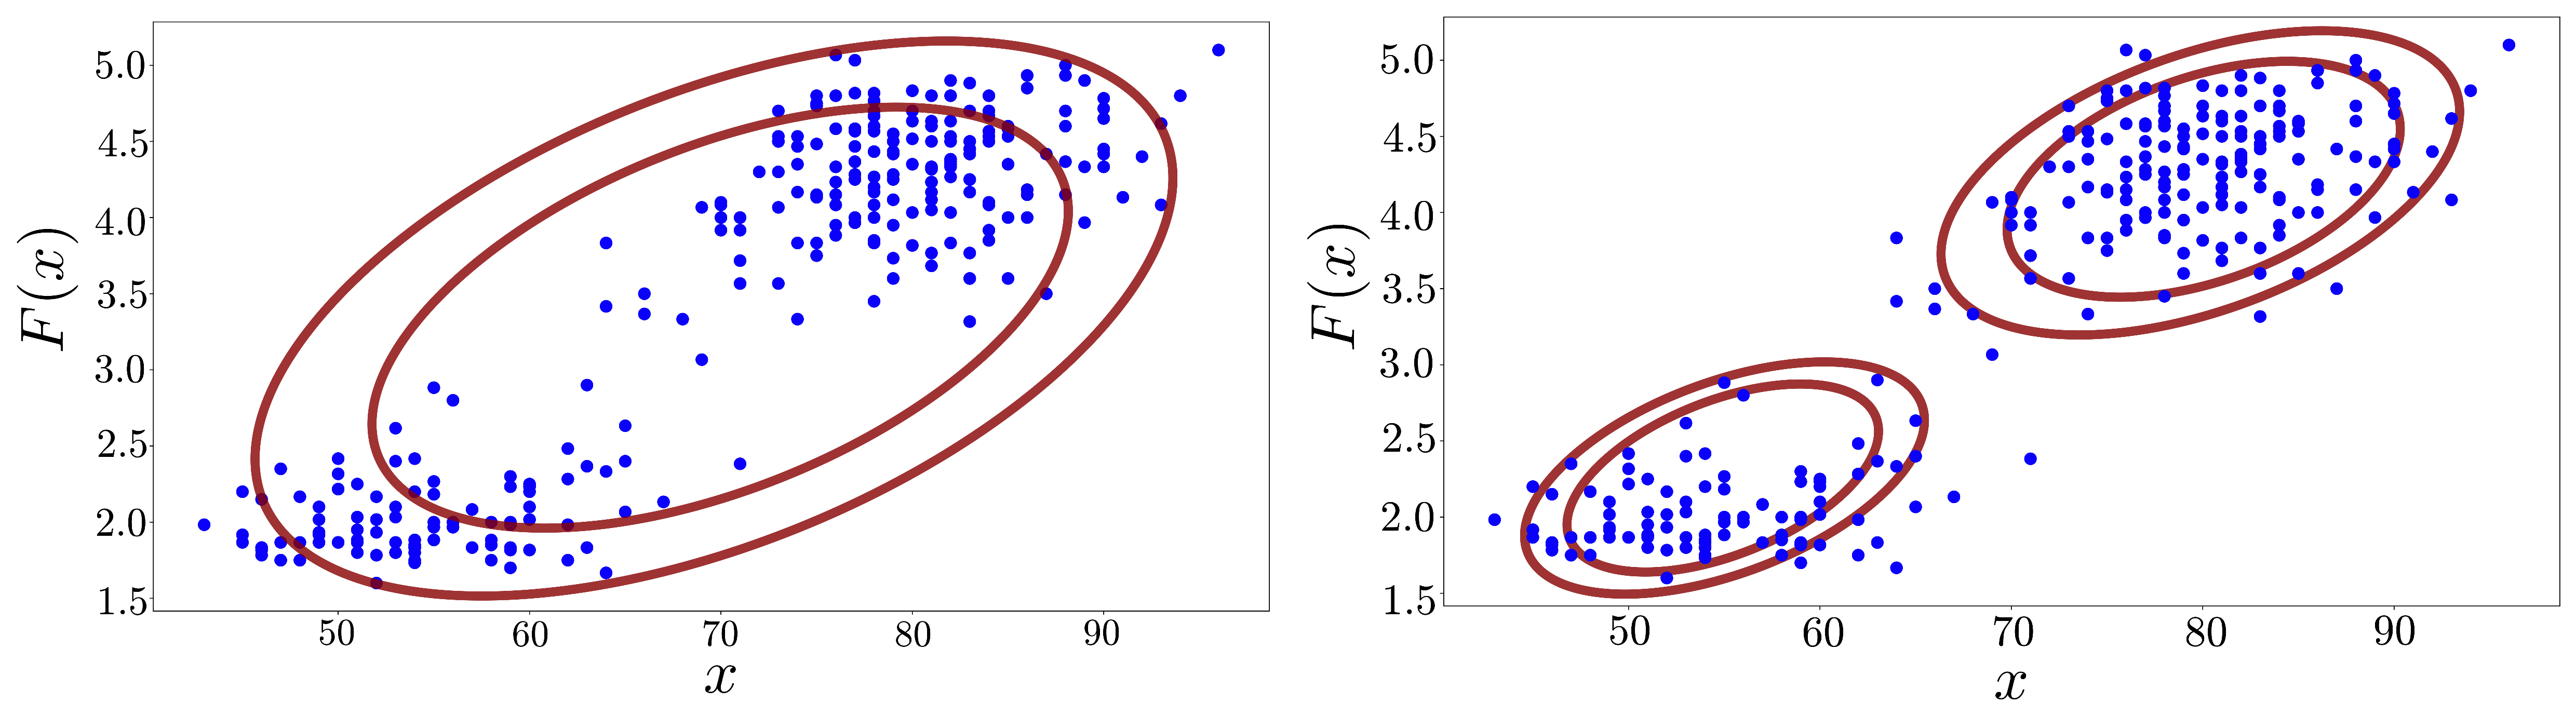
\includegraphics[width=\linewidth]{moe_background.eps}
  \subfloat[\label{one_model}Multi-modal dataset fit with one model]{\hspace{0.5\linewidth}} 
  \subfloat[\label{moes}Multi-modal dataset fit
  with MoE]{\hspace{0.5\linewidth}} \caption{Comparison of multi-modal dataset
  fit with one regression model and MoE }{\hspace{0.5\linewidth}}
  \label{fig:oldfaithful}
\end{figure}

Let $F(x; \theta)$ denote a collection of $N_F$ expert models $F(x;\theta) :=
\{F_1(x; \theta_1), \dots, \\ F_{N_{F}}(x; \theta_{N_F})\}$, whose parameters
are given by the set $\theta=\{\theta_1, \dots, \theta_{N_{F}} \}$.
%
The gating network is responsible for dividing the input space $\mathcal{X}
\subset \mathbb{R}^m$ into \textit{state partitions}, and assigning local expert
models capable of providing specialized predictions for each partition.
%
% The task of the gating network can be viewed as dividing the input space
% $\mathcal{X}$ into \textit{state partitions} within which a local expert is
% active. 
%
We represent the gating network with the discrete probability distribution
$\mathbf{P}(x| \psi) := (P_1(x| \psi), \dots, P_{N_F}(x| \psi))$, where $P_i(x |
\psi)$ denotes the probability of state $x$ belonging to the state partition
$\mathcal{X}^i \subset \mathcal{X}$ with the index $i \in \{1, \dots, N_F \}$. 
%
% The gating network behaves as a routing function that assigns
% a local expert model capable of providing specialized predictions for states
% within the partition $\mathcal{X}' \subset \mathcal{X}$ of the input space
% $\mathcal{X} \subset \mathbb{R}^{2m}$. 
%
%
In the standard MoE framework~\cite{jordan1994hierarchical}, the prediction
$u(x)$ of the MoE is given by
\begin{align}
  u(x) &= \sum_{i=1}^{N_F}F_i(x; \theta_i)P_i(x | \psi),
  \label{eq:weighted_sum}
\end{align}
%
which requires evaluating all the experts for each input $x$.
%
We can reduce the computation cost of~\eqref{eq:weighted_sum} by utilizing the
output of the single best expert as determined by the gating
network\cite{chen2022towards}
\begin{equation}
    u(x) = \{ F_a(x; \theta_a) \; | \; a = \underset{i}{\textrm{argmax}} \{ P_i(x | \psi) \} \}.
  \label{eq:best_expert_prediction}
\end{equation}
%
% which allows us to achieve comparably accurate predictions
% to~\eqref{eq:weighted_sum} with minimal computation cost\cite{chen2022towards}.
% Compared to the prediction in~\eqref{eq:weighted_sum}, the outputs from the
% single best expert provide specialized predictions capable of exhibiting
% discontinuous outputs at the boundaries of the state partitions.

\textbf{Model Structure}: The expert models and the gating network can take
several forms. 
%
Gaussian process (GP) models are commonly used in the MoE framework to infer a
multi-modal probabilistic model from a small amount of
data~\cite{harkonen2022mixtures}.
%
Despite the expressive power and tractability of GP experts, the inference
procedure requires repeated matrix inversions that scale cubically with the size
of the dataset~\cite{zhang2019embarrassingly}.  
%
% In various literature, the gating network is constructed from linear combination
% of Gaussian kernels\cite{harkonen2022mixtures} or a Dirichlet
% distribution\cite{rasmussen2001infinite}. 
% %
% Moreover, Gaussian gating networks can only provide a quadratic parameterization
% of the boundaries of the state partitions.
%
In order to circumvent the large computational and memory overhead while also
preserving the expressive power of GP experts, we leverage the universal
approximation capabilities of neural networks for both the experts and the
gating network.
%
For regression problems that require the flexibility of nonlinear models, the
experts can be given by deep neural-nets with point-estimate parameters, which
can be extended to probabilistic models with the use of Bayesian neural
networks, whose weights and biases are given by probability
distributions~\cite{jospin2020hands}.
%
Similarly, the gating network can be given by a neural network $\mathbf{P}(x| \psi) :
\mathcal{X} \rightarrow \mathbb{R}^{N_F}$ with parameters $\psi$, and the output
corresponds to the vector $[P_1(x| \psi), \dots, P_{N_F}(x| \psi)]$.
%
In order to ensure that the probabilities $P_i(x | \psi)$ over all state
partitions $i$ sum to one, we use the \textsc{Softmax} activation
function~\cite{sharma2017activation} on the last layer of the gating network.
%
% The objective is to learn the decision parameters $(\psi, \theta)$ from observed
% data.

\textbf{Training}: Given the training dataset $\mathbb{D} = \{(x_1, y_1), \dots,
(x_N, y_N)\}$ with $N$ input state-label pairs, we can use gradient-based
techniques to find the optimal parameters $(\psi, \theta)$ that best fit
the dataset~\cite{chen2022towards}.
%
In such techniques, we construct the cost function we wish to minimize as
\begin{align}
  \mathbb{L}(\mathbb{D})= \sum_{j=1}^{N} \sum_{i=1}^{N_F} \norm{F_i(x_j; \theta_i) - y_j}{} \; P_i(x_j, \psi),
  \label{eq:log_normal_likelihood}
\end{align}
\noindent where $\norm{F_i(x_j; \theta_i) - y_j}{}$ is the error in the
prediction made by the expert $i$. 
% 
% Notice that the cost function $\mathbb{L}$ measures how likely the current
% parameters $(\psi, \theta)$ are to generate the sampled data $\mathbb{D}$. 
%
Notice that the cost function~\eqref{eq:log_normal_likelihood} is minimum
when the parameter $\theta_i$ has the lowest prediction error and the highest
probability of getting selected by the gating network.
%
% We evaluate the pertinent gradients of the cost function $\nicefrac{\partial
% \mathbb{L}}{\partial \psi}, \nicefrac{\partial \mathbb{L}}{\partial \theta}$
% analytically or via auto-differentiation and update the decision parameters with
% stochastic gradient descent.
So long as the complexity of the experts and the cost function allow for the
pertinent gradients $\nicefrac{\partial \mathbb{L}}{\partial \psi},
\nicefrac{\partial \mathbb{L}}{\partial \theta}$ to be evaluated, we can
invoke stochastic gradient descent (SGD) to update the decision parameters as
follows:
\begin{align*}
  \psi \leftarrow \psi - \frac{\partial \mathbb{L}}{\partial \psi}, \\
  \theta \leftarrow \theta - \frac{\partial \mathbb{L}}{\partial \theta}.
\end{align*}

